\documentclass[10pt]{article}

%import packages
\usepackage{graphicx}

%set margins
\topmargin = 0in
\headheight = 0in
\headsep = 0in
\textwidth = 6.5in
\oddsidemargin = 0in
\evensidemargin = 0in
\footskip = 0.5 in
\textheight = 9 in
\pagestyle{plain}

%begin document
\begin{document}

\section*{Title of my lab}

\section*{A subsection title, like Introduction or something like that}

This is \emph{italics}.


This is {\bf bold}.


This is a numbered list.

\begin{enumerate}
	\item Number one.
	\item Number two.
	\item Number three.
\end{enumerate}

This is a bulleted list.

\begin{itemize}
	\item first bullet.
	\item second bullet.
\end{itemize}

This is an image. The image should be jpg or pdf. You can use add a caption. Notice that it's centered. You can refer to it as Figure \ref{uniqueLabel} using a reference. Be sure to put a unique label with the reference.

\begin{figure}[htbp]
\begin{center}
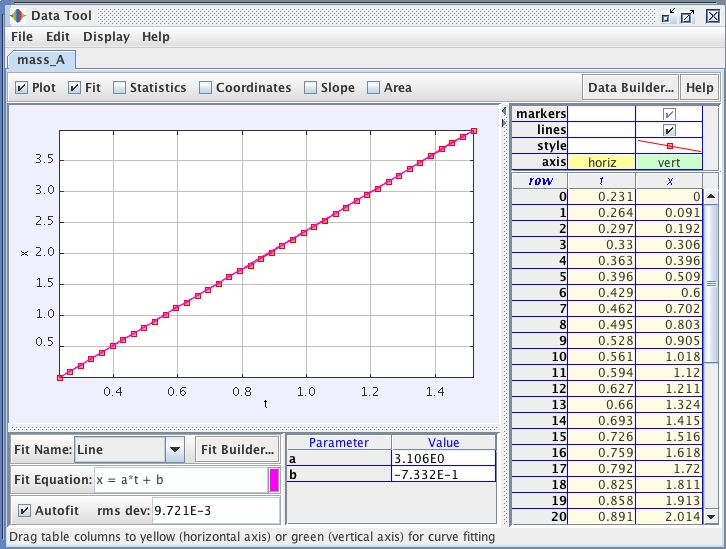
\includegraphics[scale=0.3]{imagename}
\caption{This is the caption.}
\label{uniqueLabel}
\end{center}
\end{figure}

This is a numbered equation.

\begin{equation}
	\vec{F}_{net}=\frac{d\vec{p}}{dt}
\end{equation}

This is an equation which isn't numbered.

\begin{displaymath}
	\vec{v}=\left< v_x, v_y, v_z \right>
\end{displaymath}

If you want to type math characters in a sentence like $\omega = 2\pi / T$ then you do it like this.

\end{document}